\documentclass{article}
\usepackage[utf8]{inputenc}
\usepackage{lmodern}
\usepackage[T1]{fontenc}
\usepackage[spanish,activeacute]{babel}
\usepackage{titlesec}
\titleformat{\section}
  {\normalfont\fontsize{14}{14}\bfseries}{\thesection}{1em}{}
\titlespacing{\paragraph}{0pt}{1.5em}{.5em}[]

\usepackage{mathtools}
\usepackage{graphicx}
\DeclareGraphicsExtensions{.png,.pdf,.jpg}
\usepackage{float}
\usepackage{amssymb}
\usepackage{cancel}
\usepackage{bm}
\usepackage{amsmath}

\usepackage{listings}
\usepackage{color}
\usepackage{hyperref}

\definecolor{dkgreen}{rgb}{0,0.6,0}
\definecolor{gray}{rgb}{0.5,0.5,0.5}
\definecolor{mauve}{rgb}{0.58,0,0.82}

\lstset{frame=tb,
  language=Java,
  aboveskip=3mm,
  belowskip=3mm,
  showstringspaces=false,
  columns=flexible,
  basicstyle={\small\ttfamily},
  numbers=none,
  numberstyle=\tiny\color{gray},
  keywordstyle=\color{blue},
  commentstyle=\color{dkgreen},
  stringstyle=\color{mauve},
  breaklines=true,
  breakatwhitespace=true,
  tabsize=3
}
\hypersetup{
    colorlinks,
    citecolor=black,
    filecolor=black,
    linkcolor=black,
    urlcolor=black
}
\title{Taller de Coches}
\author{Martin Fagoaga y Gonzalo Álvarez}
\date{2022}
\begin{document}
\maketitle 
\clearpage
\tableofcontents
\clearpage
\listoffigures
\clearpage

\section{FASE 1: ANALISIS Y DISEÑO}
\subsection{Introducción: AppTaller}
\subsection{Objetivos}
\subsection{Contextualización del proyecto}
\subsection{Análisis}
\subsection{Diseño} 
\begin{figure}[H]
  \centering
  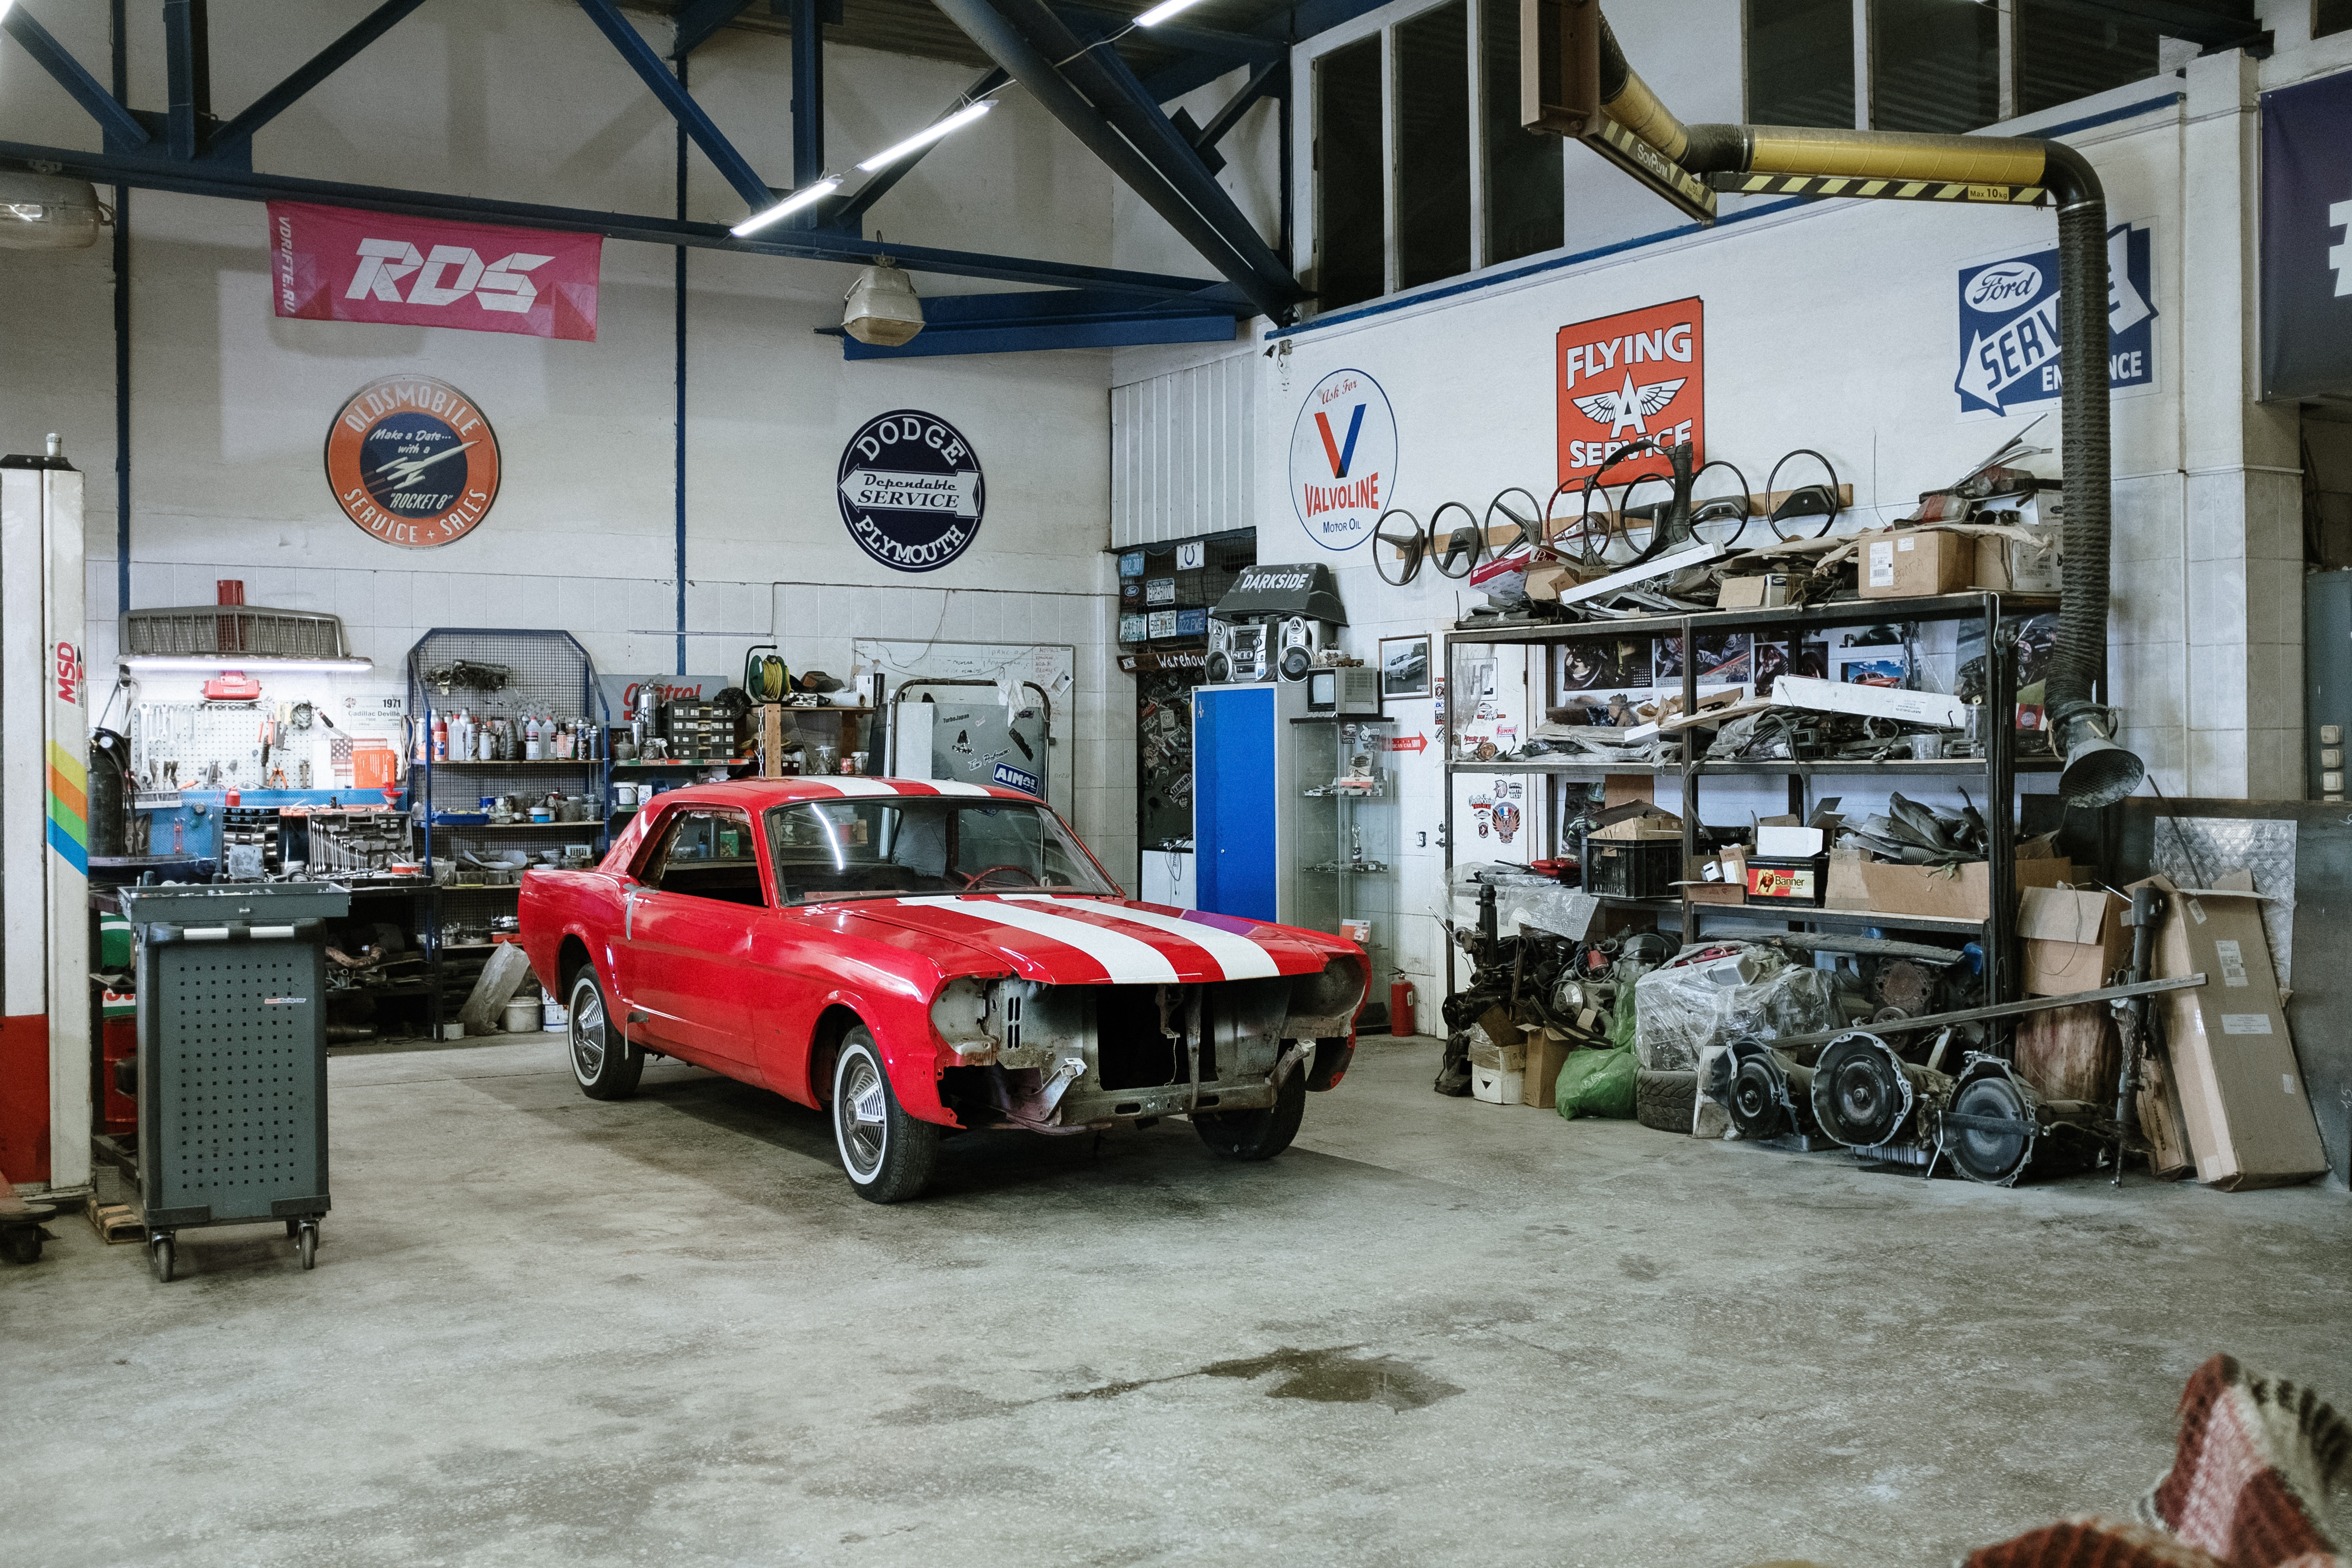
\includegraphics[width=1.0\textwidth]{pexels-cottonbro-4480505.jpg}
  \caption{Diagrama de casos de uso}
\end{figure}
\subsection{Planificación semanal}
\subsection{FOL}
\section{FASE 2: IMPLEMENTACIÓN Y PRUEBAS}
\subsection{DDBB: Código SQL}
\lstset{%
  	backgroundcolor=\color{white},
      inputencoding=utf8,
    escapeinside={\%*}{*)},
    literate={á}{{\'a}}1 {é}{{\'e}}1 {í}{{\'i}}1 {ó}{{\'o}}1 {ú}{{\'u}}1 {Á}{{\'A}}1 {É}{{\'E}}1 {Í}{{\'I}}1 {Ó}{{\'O}}1 {Ú}{{\'U}}1 {ñ}{{\~n}}1 {Ñ}{{\~N}}1,
  	basicstyle=\footnotesize,
  	breakatwhitespace=false,
  	breaklines=true,
  	captionpos=b,
  	commentstyle=\color{dkgreen},
  	deletekeywords={...},
  	escapeinside={\%*}{*)},
  	extendedchars=true,
  	frame=single,
  	keepspaces=true,
  	keywordstyle=\color{blue},
  	language=SQL,
  	morekeywords={*,modify,MODIFY,...},
  	numbers=left,
  	numbersep=15pt,
  	numberstyle=\tiny,
  	rulecolor=\color{ltgray},
  	showspaces=false,
  	showstringspaces=false, 
  	showtabs=false,
  	stepnumber=1,
  	tabsize=3,
}
\begin{lstlisting}[caption=Script .sql para crear la BD (BBDD)]
    /*Creamos tablespaces*/
create tablespace administracion datafile 'administracion.dbf' size 1M autoextend on;
create tablespace taller datafile 'taller.dbf' size 1M autoextend on;

/*Creamos los usuarios*/
create user Jefe identified by "jefe_1daw3_chuleta";
alter user Jefe default tablespace administracion;
create user mech1 identified by "mech1";
alter user mech1 default tablespace taller;
create user mech2 identified by "mech2";
alter user mech2 default tablespace taller;
create user mech3 identified by "mech3";
alter user mech3 default tablespace taller;
create user mech4 identified by "mech4";
alter user mech4 default tablespace taller;
create user mech5 identified by "mech5";
alter user mech5 default tablespace taller;
create user websiteVisit identified by "webVisitor";


/*Modificamos los perfiles por defecto para que no pidan cambiar password*/
alter profile default limit PASSWORD_REUSE_TIME UNLIMITED;
alter profile DEFAULT LIMIT PASSWORD_LIFE_TIME UNLIMITED;

/*Modificamos perfil de los mecanicos, maximo 1 sesion por usuario*/
create profile sesiones_mecanico LIMIT
sessions_per_user 1
failed_login_attempts UNLIMITED;
alter user mech1 PROFILE sesiones_mecanico;
alter user mech2 PROFILE sesiones_mecanico;
alter user mech3 PROFILE sesiones_mecanico;
alter user mech4 PROFILE sesiones_mecanico;
alter user mech5 PROFILE sesiones_mecanico;

/*Modificamos perfil de visitante web*/
create profile sesiones_web LIMIT
sessions_per_user UNLIMITED;
alter user websiteVisit PROFILE sesiones_web;


/*Cremos las tablas, triggers y costraints*/
create table CLIENTE(
    ID_CLIENTE NUMBER(10) PRIMARY KEY,
    NOMBRE VARCHAR2(20) NOT NULL,
    APELLIDO VARCHAR2(30) NOT NULL,
    TELEFONO VARCHAR2(9) NOT NULL,
    DIRECCION VARCHAR2(40),
    DNI VARCHAR2(9) UNIQUE,
    CORREO VARCHAR2(20) UNIQUE
) tablespace taller;
create public synonym CLIENTE for system.CLIENTE;
CREATE SEQUENCE CLIENTES_SEQ START WITH 1;

CREATE OR REPLACE TRIGGER CLIENTES_IDS BEFORE INSERT ON CLIENTE FOR EACH ROW
BEGIN SELECT CLIENTES_SEQ.NEXTVAL INTO :NEW.ID_CLIENTE FROM DUAL;
END;
/


create table VEHICULO(
    ID_VEHICULO NUMBER(10) PRIMARY KEY,
    MODELO VARCHAR2(20),
    COLOR VARCHAR2(10),
    AÑO DATE,
    MATRICULA VARCHAR2(7) UNIQUE,
    ID_CLIENTE NUMBER(10)
) tablespace taller;
create public synonym VEHICULO for system.VEHICULO;
CREATE SEQUENCE VEHICULOS_SEQ START WITH 1;

CREATE OR REPLACE TRIGGER VEHICULOS_IDS BEFORE INSERT ON VEHICULO FOR EACH ROW
BEGIN SELECT VEHICULOS_SEQ.NEXTVAL INTO :NEW.ID_VEHICULO FROM DUAL;
END;
/


create table FACTURA(
    ID_FACTURA NUMBER(10) PRIMARY KEY,
    FECHA_ENTRADA DATE,
    PRECIO_TOTAL NUMBER(5,2),
    FECHA_FIN DATE,
    PAGADO NUMBER(1,0),
    ID_VEHICULO NUMBER(10)
) tablespace taller;
create public synonym FACTURA for system.FACTURA;
CREATE SEQUENCE FACTURA_SEQ START WITH 1;
CREATE OR REPLACE TRIGGER FACTURAS_IDS BEFORE INSERT ON FACTURA FOR EACH ROW
BEGIN SELECT FACTURA_SEQ.NEXTVAL INTO :NEW.ID_FACTURA FROM DUAL;
END;
/

create table REPARACION(
    ID_REPARACION NUMBER(10) PRIMARY KEY,
    TIEMPO_HORA DATE,
    HORAS_DURACION NUMBER(4,2),
    COMENTARIOS VARCHAR2(300),
    ID_FACTURA NUMBER(10)

) tablespace taller;
create public synonym REPARACION for system.reparacion;
CREATE SEQUENCE REPARACION_SEQ START WITH 1;
CREATE OR REPLACE TRIGGER REPARACION_IDS BEFORE INSERT ON REPARACION FOR EACH ROW
BEGIN SELECT REPARACION_SEQ.NEXTVAL INTO :NEW.ID_REPARACION FROM DUAL;
END;
/

create table piezas(
    ID_PIEZA NUMBER(10) PRIMARY KEY,
    MARCA VARCHAR2(20),
    MODELO VARCHAR2(50),
    PRECIO NUMBER(5,2),
    STOCK NUMBER(3),
    DESCRIPCION VARCHAR2(255),
    URL VARCHAR2(255),
    ID_CATEGORIA NUMBER(10)
) tablespace taller;
create public synonym PIEZAS for system.piezas;
CREATE SEQUENCE PIEZAS_SEQ START WITH 1;
CREATE OR REPLACE TRIGGER PIEZAS_IDS BEFORE INSERT ON PIEZAS FOR EACH ROW
BEGIN SELECT PIEZAS_SEQ.NEXTVAL INTO :NEW.ID_PIEZA FROM DUAL;
END;
/

create table categorias(
    ID_CATEGORIA NUMBER(10) PRIMARY KEY,
    NOMBRE VARCHAR2(40) UNIQUE
) tablespace taller;
create public synonym CATEGORIAS for system.CATEGORIAS;
CREATE SEQUENCE CATEGORIAS_SEQ START WITH 1;
CREATE OR REPLACE TRIGGER CATEGORIAS_IDS BEFORE INSERT ON CATEGORIAS FOR EACH ROW
BEGIN SELECT CATEGORIAS_SEQ.NEXTVAL INTO :NEW.ID_CATEGORIA FROM DUAL;
END;
/

create table usa(
    ID_PIEZA NUMBER(10),
    ID_REPARACION NUMBER(10),
    CANTIDAD NUMBER(3)
) tablespace taller;
create public synonym USA for system.USA;

create table Realiza(
    ID_REPARACION NUMBER(10),
    ID_EMPLEADO NUMBER(10)

) tablespace taller;
create public synonym REALIZA for system.Realiza;

create table empleado(
    ID_EMPLEADO NUMBER(10) PRIMARY KEY,
    NOMBRE VARCHAR2(10),
    APELLIDO VARCHAR2(30),
    TELEFONO VARCHAR2(9),
    DNI VARCHAR2(9) UNIQUE,
    ID_JEFE NUMBER(10)
)tablespace administracion;
create public synonym EMPLEADO for system.empleado;
CREATE SEQUENCE EMPLEADO_SEQ START WITH 1;
CREATE OR REPLACE TRIGGER EMPLEADOS_IDS BEFORE INSERT ON EMPLEADO FOR EACH ROW
BEGIN SELECT EMPLEADO_SEQ.NEXTVAL INTO :NEW.ID_EMPLEADO FROM DUAL;
END;
/

ALTER TABLE VEHICULO ADD CONSTRAINT VEHICULO_FK FOREIGN KEY (ID_CLIENTE) REFERENCES CLIENTE(ID_CLIENTE);
ALTER TABLE FACTURA ADD CONSTRAINT FACTURA_FK FOREIGN KEY (ID_VEHICULO) REFERENCES VEHICULO(ID_VEHICULO);
ALTER TABLE REPARACION ADD CONSTRAINT REP_FK FOREIGN KEY (ID_FACTURA) REFERENCES FACTURA(ID_FACTURA);
ALTER TABLE EMPLEADO ADD CONSTRAINT EMP_FK FOREIGN KEY (ID_JEFE) REFERENCES EMPLEADO(ID_EMPLEADO);
ALTER TABLE PIEZAS ADD CONSTRAINT PIEZAS_FK FOREIGN KEY (ID_CATEGORIA) REFERENCES CATEGORIAS(ID_CATEGORIA);
ALTER TABLE PIEZAS ADD CONSTRAINT COMBO_UNIC UNIQUE (MARCA,MODELO);
ALTER TABLE USA ADD CONSTRAINT USA_PK PRIMARY KEY (ID_PIEZA,ID_REPARACION);
ALTER TABLE USA ADD CONSTRAINT USA_FK1 FOREIGN KEY (ID_PIEZA) REFERENCES PIEZAS(ID_PIEZA);
ALTER TABLE USA ADD CONSTRAINT USA_FK2 FOREIGN KEY (ID_REPARACION) REFERENCES REPARACION(ID_REPARACION);
ALTER TABLE REALIZA ADD CONSTRAINT REALIZA_PK PRIMARY KEY (ID_EMPLEADO,ID_REPARACION);
ALTER TABLE REALIZA ADD CONSTRAINT REALIZA_FK1 FOREIGN KEY (ID_EMPLEADO) REFERENCES EMPLEADO(ID_EMPLEADO);
ALTER TABLE REALIZA ADD CONSTRAINT REALIZA_FK2 FOREIGN KEY (ID_REPARACION) REFERENCES REPARACION(ID_REPARACION);


ALTER TABLE CLIENTE ADD CONSTRAINT DNI_FORM CHECK (REGEXP_LIKE(DNI,'\d{8}[A-Z]$'));
ALTER TABLE CLIENTE ADD CONSTRAINT TEL_FORM CHECK (REGEXP_LIKE(TELEFONO,'\d{9}'));
ALTER TABLE CLIENTE ADD CONSTRAINT CORREO_FORM CHECK (REGEXP_LIKE(CORREO,'[A-Za-zá-ú0-9_.]*@[A-Za-zá-ú0-9_]*.[A-Za-z]*$'));
ALTER TABLE EMPLEADO ADD CONSTRAINT EMP_DNI_FORM CHECK (REGEXP_LIKE(DNI,'\d{8}[A-Z]$'));
ALTER TABLE EMPLEADO ADD CONSTRAINT EMP_TEL_FORM CHECK (REGEXP_LIKE(TELEFONO,'\d{9}'));
/*ALTER TABLE VEHICULO ADD CONSTRAINT MATR_FORM CHECK (REGEXP_LIKE(MATRICULA, ''))
*/


/*Creamos roles para usuario de administracion y mecanico, y los asignamos*/
create role rol_administrador;
grant all privileges to rol_administrador;
create role rol_mecanico;
grant create SESSION to rol_mecanico;
grant update (Stock) on Piezas to rol_mecanico;
grant insert on Piezas to rol_mecanico;
grant select on Piezas to rol_mecanico;
grant all on CLIENTE to rol_mecanico;
revoke delete on CLIENTE from rol_mecanico;
grant all on Vehiculo to rol_mecanico;
revoke delete on Vehiculo from rol_mecanico;
grant all on Factura to rol_mecanico;
revoke delete on Factura from rol_mecanico;
grant all on Reparacion to rol_mecanico;
grant all on Usa to rol_mecanico;
revoke delete on Usa from rol_mecanico;
grant all on categorias to rol_mecanico;
revoke delete on categorias from rol_mecanico;
grant insert on Realiza to rol_mecanico;
grant select on EMPLEADO to rol_mecanico;

grant select on piezas to websiteVisit;
grant select on categorias to websiteVisit;

grant rol_administrador to Jefe;
grant rol_mecanico to mech1;
grant rol_mecanico to mech2;
grant rol_mecanico to mech3;
grant rol_mecanico to mech4;
grant rol_mecanico to mech5;
alter user mech1 DEFAULT role rol_mecanico;
alter user mech2 DEFAULT role rol_mecanico;
alter user mech3 DEFAULT role rol_mecanico;
alter user mech4 DEFAULT role rol_mecanico;
alter user mech5 DEFAULT role rol_mecanico;



/*Inserts*/

/*Categorias*/
INSERT INTO CATEGORIAS(NOMBRE)VALUES('Filtros y Aceite');
INSERT INTO CATEGORIAS(NOMBRE)VALUES('Frenado');
INSERT INTO CATEGORIAS(NOMBRE)VALUES('Embrague y caja de cambios');
INSERT INTO CATEGORIAS(NOMBRE)VALUES('Óptica Faros Bombillas');
INSERT INTO CATEGORIAS(NOMBRE)VALUES('Arranque y carga');
INSERT INTO CATEGORIAS(NOMBRE)VALUES('Accesorios y Equipamiento');
INSERT INTO CATEGORIAS(NOMBRE)VALUES('Piezas Motor');



INSERT INTO PIEZAS(MARCA,MODELO,PRECIO,STOCK,DESCRIPCION,URL,ID_CATEGORIA)VALUES(
'SHELL','Helix HX8 5W40 SN 3* 5L A518', 25.50 , 10, 'Aceite de motor (aceite motor)','https://oscaro.media/catalog/images/oscjpg/zoom/1010/5l_helix_hx8_syn_5w_40_high.jpg',1);
INSERT INTO PIEZAS(MARCA,MODELO,PRECIO,STOCK,DESCRIPCION,URL,ID_CATEGORIA)VALUES(
'PETRONAS','SYNTIUM 5000 XS 5W-30 SN 4X5L', 28.90 , 21, 'Aceite de motor (aceite motor)','https://oscaro.media/catalog/images/osc360/11868700/Lv2/img19.jpg',1);
INSERT INTO PIEZAS(MARCA,MODELO,PRECIO,STOCK,DESCRIPCION,URL,ID_CATEGORIA)VALUES(
'MOBIL','Super 2000 10W40 5+1L', 34.60 , 14, 'Aceite de motor (aceite motor)','https://oscaro.media/catalog/images/oscjpg/zoom/1013/151476-51.jpg',1);
INSERT INTO PIEZAS(MARCA,MODELO,PRECIO,STOCK,DESCRIPCION,URL,ID_CATEGORIA)VALUES(
'OSCARO','5W40', 21.70 , 10, 'Aceite de motor (aceite motor)','https://oscaro.media/catalog/images/osc360/12551004/Lv2/img23.jpg',1);
INSERT INTO PIEZAS(MARCA,MODELO,PRECIO,STOCK,DESCRIPCION,URL,ID_CATEGORIA)VALUES(
'CASTROL','CASTROL Magnatec 10W-40', 29.70 , 120, 'Aceite de motor (aceite motor)','https://oscaro.media/catalog/images/oscjpg/zoom/1012/15ca1f.jpg',1);
INSERT INTO PIEZAS(MARCA,MODELO,PRECIO,STOCK,DESCRIPCION,URL,ID_CATEGORIA)VALUES(
'TOTALENERGIES','QUARTZ 9000 5W40', 33.90 , 40, 'Aceite de motor (aceite motor)','https://oscaro.media/catalog/images/oscjpg/zoom/1029/213678.jpg',1);
INSERT INTO PIEZAS(MARCA,MODELO,PRECIO,STOCK,DESCRIPCION,URL,ID_CATEGORIA)VALUES(
'ELF','EVOLUTION 900 5W40', 32.60 , 52, 'Aceite de motor (aceite motor)','https://oscaro.media/catalog/images/osc360/12549869/Lv2/img23.jpg',1);
INSERT INTO PIEZAS(MARCA,MODELO,PRECIO,STOCK,DESCRIPCION,URL,ID_CATEGORIA)VALUES(
'MOBIL','Super 2000 Formula P 10W40', 31.90 , 50, 'Aceite de motor (aceite motor)','https://oscaro.media/catalog/images/osc360/4625490/Lv2/img23.jpg',1);
INSERT INTO PIEZAS(MARCA,MODELO,PRECIO,STOCK,DESCRIPCION,URL,ID_CATEGORIA)VALUES(
'PETRONAS','SYNTIUM 7000 XS 5W30', 10.90 , 30, 'Aceite de motor (aceite motor)','https://oscaro.media/catalog/images/osc360/11868675/Lv2/img05.jpg',1);
INSERT INTO PIEZAS(MARCA,MODELO,PRECIO,STOCK,DESCRIPCION,URL,ID_CATEGORIA)VALUES(
'PETRONAS','SYNTIUM 5000 XS 5W30', 34.90 , 40, 'Aceite de motor (aceite motor)','https://oscaro.media/catalog/images/osc360/11868700/Lv2/img23.jpg',1);
    

insert into PIEZAS(MARCA,MODELO,PRECIO,STOCK,DESCRIPCION,URL,ID_CATEGORIA)VALUES ('BOSCH','0 986 494 204',44.80,4,'Juego de 4 pastillas de freno (zapata)','https://oscaro.media/catalog/images/jpg/zoom/30/0986494204phrewhco0000.jpg',2);
insert into PIEZAS(MARCA,MODELO,PRECIO,STOCK,DESCRIPCION,URL,ID_CATEGORIA)VALUES ('BREMBO','08.2536.10',85.80,4,'Discos de freno','https://oscaro.media/catalog/images/jpg/zoom/65/08253610.jpg',2);
insert into PIEZAS(MARCA,MODELO,PRECIO,STOCK,DESCRIPCION,URL,ID_CATEGORIA)VALUES ('BUDWEG CALIPER A/S','343520',121.50,3,'Pinza de freno, reacondicionada.','https://oscaro.media/catalog/images/oscjpg/zoom/114/343520.jpg',2);
insert into PIEZAS(MARCA,MODELO,PRECIO,STOCK,DESCRIPCION,URL,ID_CATEGORIA)VALUES ('BOSCH','0 986 134 428',164.90,5,'Pinza de freno','https://oscaro.media/catalog/images/jpg/zoom/30/0986134428phfrwhco0000.jpg',2);
insert into PIEZAS(MARCA,MODELO,PRECIO,STOCK,DESCRIPCION,URL,ID_CATEGORIA)VALUES ('METZGER','6250252',75.80,2,'Pinza de freno','https://oscaro.media/catalog/images/bmp/zoom/94/6250252.jpg',2);
insert into PIEZAS(MARCA,MODELO,PRECIO,STOCK,DESCRIPCION,URL,ID_CATEGORIA)VALUES ('FEBI BILSTEIN','102296',35.40,1,'Sensor, revoluciones de la rueda','https://oscaro.media/catalog/images/jpg/zoom/101/102296_1.jpg',2);
insert into PIEZAS(MARCA,MODELO,PRECIO,STOCK,DESCRIPCION,URL,ID_CATEGORIA)VALUES ('AJUSA','01107400',5.9,4,'Junta (retén)','https://oscaro.media/catalog/images/oscjpg/zoom/139/01107400.jpg',2);
insert into PIEZAS(MARCA,MODELO,PRECIO,STOCK,DESCRIPCION,URL,ID_CATEGORIA)VALUES ('ELRING','646.830',24.10,4,'Junta, bomba de vacío','https://oscaro.media/catalog/images/oscjpg/zoom/10/758044.jpg',2);
insert into PIEZAS(MARCA,MODELO,PRECIO,STOCK,DESCRIPCION,URL,ID_CATEGORIA)VALUES ('BREMBO','09.8304.21',64.60,4,'Discos de freno','https://oscaro.media/catalog/images/jpg/zoom/65/09830421.jpg',2);

insert into PIEZAS(MARCA,MODELO,PRECIO,STOCK,DESCRIPCION,URL,ID_CATEGORIA)VALUES ('LUK','602 0008 00',981.50,1,'Kit de embrague','https://oscaro.media/catalog/images/jpg/zoom/6/602000800.jpg',3);
insert into PIEZAS(MARCA,MODELO,PRECIO,STOCK,DESCRIPCION,URL,ID_CATEGORIA)VALUES ('VALEO','828060',349.90,4,'Kit de embrague','https://oscaro.media/catalog/images/jpg/zoom/21/valeo_kit3p_rb.jpg',3);
insert into PIEZAS(MARCA,MODELO,PRECIO,STOCK,DESCRIPCION,URL,ID_CATEGORIA)VALUES ('LUK','624 3474 09',230.90,2,'Kit de embrague','https://oscaro.media/catalog/images/jpg/zoom/6/09_luk_pc_single_parts_clutch.jpg',3);
insert into PIEZAS(MARCA,MODELO,PRECIO,STOCK,DESCRIPCION,URL,ID_CATEGORIA)VALUES ('VALEO','821362',136.90,4,'Kit de embrague','https://oscaro.media/catalog/images/jpg/zoom/21/821362c.jpg',3);
insert into PIEZAS(MARCA,MODELO,PRECIO,STOCK,DESCRIPCION,URL,ID_CATEGORIA)VALUES ('BLUE PRINT','ADA103012',246.90,3,'Kit de embrague','https://oscaro.media/catalog/images/jpg/zoom/350/ada103012_2.jpg',3);
insert into PIEZAS(MARCA,MODELO,PRECIO,STOCK,DESCRIPCION,URL,ID_CATEGORIA)VALUES ('AISIN','ATF-91005',51.40,3,'Aceite caja de cambios','https://oscaro.media/catalog/images/jpg/zoom/166/atf-91005%2001.jpg',3);
insert into PIEZAS(MARCA,MODELO,PRECIO,STOCK,DESCRIPCION,URL,ID_CATEGORIA)VALUES ('AISIN','CVTF-90005',53.90,2,'Aceite caja de cambios','https://oscaro.media/catalog/images/jpg/zoom/166/cvtf-90005%2001.jpg',3);
insert into PIEZAS(MARCA,MODELO,PRECIO,STOCK,DESCRIPCION,URL,ID_CATEGORIA)VALUES ('SHELL','Spirax S4G75W80',9.60,1,'Aceite caja de cambios','https://oscaro.media/catalog/images/oscjpg/zoom/1010/spirax_s4_g_75w-80%20(1).jpg',3);
insert into PIEZAS(MARCA,MODELO,PRECIO,STOCK,DESCRIPCION,URL,ID_CATEGORIA)VALUES ('CORTECO','20034710B',13.70,12,'Casquilo guía, embrague','https://oscaro.media/catalog/images/bmp/zoom/140/20034710.jpg',3);
insert into PIEZAS(MARCA,MODELO,PRECIO,STOCK,DESCRIPCION,URL,ID_CATEGORIA)VALUES ('FEBI BILSTEIN','46008',20.90,4,'Casquilo guía, embrague','https://oscaro.media/catalog/images/jpg/zoom/101/46008_1.jpg',3);


insert into PIEZAS(MARCA,MODELO,PRECIO,STOCK,DESCRIPCION,URL,ID_CATEGORIA)VALUES ('VALEO','046871',728.50,1,'Faro principal (faro delantero)','https://oscaro.media/catalog/images/jpg/zoom/21/valeo_headlamp_046871_01.jpg',4);
insert into PIEZAS(MARCA,MODELO,PRECIO,STOCK,DESCRIPCION,URL,ID_CATEGORIA)VALUES ('VAN WEZEL','2730961',34.80,4,'Faro principal (faro delantero)','https://oscaro.media/catalog/images/bmp/zoom/36/k2730961.jpg',4);
insert into PIEZAS(MARCA,MODELO,PRECIO,STOCK,DESCRIPCION,URL,ID_CATEGORIA)VALUES ('MAGNETI MARELLI','711307024171',532.90,2,'Faro principal (faro delantero)','https://oscaro.media/catalog/images/jpg/zoom/95/ilf_lpo101_wr.jpg',4);
insert into PIEZAS(MARCA,MODELO,PRECIO,STOCK,DESCRIPCION,URL,ID_CATEGORIA)VALUES ('VALEO','045437',149.90,2,'Faro principal (faro delantero)','https://oscaro.media/catalog/images/jpg/zoom/21/valeo_headlamp_045437_01.jpg',4);
insert into PIEZAS(MARCA,MODELO,PRECIO,STOCK,DESCRIPCION,URL,ID_CATEGORIA)VALUES ('VAN WEZEL','5216962',70.20,4,'Faro principal (faro delantero)','https://oscaro.media/catalog/images/bmp/zoom/36/k5216961.jpg',4);
insert into PIEZAS(MARCA,MODELO,PRECIO,STOCK,DESCRIPCION,URL,ID_CATEGORIA)VALUES ('HERTH+BUSS ELPARTS','89901311',17.40,2,'Lámpara incandescente, luz trasera (bombilla) x10','https://oscaro.media/catalog/images/jpg/normal/72/89901311.jpg',4);
insert into PIEZAS(MARCA,MODELO,PRECIO,STOCK,DESCRIPCION,URL,ID_CATEGORIA)VALUES ('PHILIPS','69741430',11.10,4,'Lámpara (bombilla). 2 x WY21 W VISION','https://oscaro.media/catalog/images/oscjpg/zoom/75/philips_pack_pr_wy21w_69741430_12071b2_s_emea_16.jpg',4);
insert into PIEZAS(MARCA,MODELO,PRECIO,STOCK,DESCRIPCION,URL,ID_CATEGORIA)VALUES ('HELLA','8GH 008 417-001',6.60,15,'Lámpara (bombilla) x 10','https://oscaro.media/catalog/images/jpg/zoom/2/k1948.jpg',4);
insert into PIEZAS(MARCA,MODELO,PRECIO,STOCK,DESCRIPCION,URL,ID_CATEGORIA)VALUES ('OSRAM','64132ULT-02B',11.60,10,'Lámpara (bombilla) 2 x H6W ULTRA LIFE','https://oscaro.media/catalog/images/jpg/zoom/67/617121-p.jpg',4);
insert into PIEZAS(MARCA,MODELO,PRECIO,STOCK,DESCRIPCION,URL,ID_CATEGORIA)VALUES ('PHILIPS','5547730',2.10,1,'Lámpara (bombilla) 2 x R10W VISION','https://oscaro.media/catalog/images/oscjpg/zoom/75/philips_pack_pr_r10w_05547730_12814b2_s_emea_16.jpg',4);

insert into PIEZAS(MARCA,MODELO,PRECIO,STOCK,DESCRIPCION,URL,ID_CATEGORIA)VALUES ('TUDOR','TB450',89.90,1,'Batería 45 Ah','https://oscaro.media/catalog/images/jpg/zoom/212/tb450new%20copie.jpg',5);
insert into PIEZAS(MARCA,MODELO,PRECIO,STOCK,DESCRIPCION,URL,ID_CATEGORIA)VALUES ('NIPPON','U540L17B',76.80,10,'Batería 50 Ah','https://oscaro.media/catalog/images/jpg/zoom/440/u540l17ba.jpg',5);
insert into PIEZAS(MARCA,MODELO,PRECIO,STOCK,DESCRIPCION,URL,ID_CATEGORIA)VALUES ('YUASA','YBX5335',89.90,1,'Batería 100 Ah','https://oscaro.media/catalog/images/oscjpg/zoom/4451/yuasaybx5335.jpg',5);
insert into PIEZAS(MARCA,MODELO,PRECIO,STOCK,DESCRIPCION,URL,ID_CATEGORIA)VALUES ('NIPPON','U540L05B',64.90,0,'Batería 35 Ah','https://oscaro.media/catalog/images/jpg/zoom/440/u540l05ba.jpg',5);
insert into PIEZAS(MARCA,MODELO,PRECIO,STOCK,DESCRIPCION,URL,ID_CATEGORIA)VALUES ('VARTA','5401260333132',66.90,4,'Batería 40 Ah','https://oscaro.media/catalog/images/jpg/zoom/26/540126033_jpg.jpg',5);
insert into PIEZAS(MARCA,MODELO,PRECIO,STOCK,DESCRIPCION,URL,ID_CATEGORIA)VALUES ('YUASA','YBX5334',96.90,2,'Batería 100 Ah','https://oscaro.media/catalog/images/jpg/zoom/4451/img_929_4871367.jpg',5);
insert into PIEZAS(MARCA,MODELO,PRECIO,STOCK,DESCRIPCION,URL,ID_CATEGORIA)VALUES ('YUASA','YBX3054',52.60,1,'Batería 36 Ah','https://oscaro.media/catalog/images/jpg/zoom/4451/img_954_4131630.jpg',5);
insert into PIEZAS(MARCA,MODELO,PRECIO,STOCK,DESCRIPCION,URL,ID_CATEGORIA)VALUES ('BOSCH','0 092 S4E 420',147.90,2,'Batería 85 Ah','https://oscaro.media/catalog/images/jpg/zoom/30/0092s4e420dranwhco00mm.jpg',5);
insert into PIEZAS(MARCA,MODELO,PRECIO,STOCK,DESCRIPCION,URL,ID_CATEGORIA)VALUES ('BOSCH','0 092 S4E 400',125.50,1,'Batería 65 Ah','https://oscaro.media/catalog/images/jpg/zoom/30/0092s4e400dranwhgr00mm.jpg',5);
insert into PIEZAS(MARCA,MODELO,PRECIO,STOCK,DESCRIPCION,URL,ID_CATEGORIA)VALUES ('VARTA','5954040833132',153.50,1,'Batería 95 Ah','https://oscaro.media/catalog/images/oscjpg/zoom/26/595404083.jpg',5);

insert into PIEZAS(MARCA,MODELO,PRECIO,STOCK,DESCRIPCION,URL,ID_CATEGORIA)VALUES ('DBS','01763194',59.90,2,'Alfombrilla a medida','https://oscaro.media/catalog/images/oscjpg/zoom/1052/tapis_star_1.jpg',6);
insert into PIEZAS(MARCA,MODELO,PRECIO,STOCK,DESCRIPCION,URL,ID_CATEGORIA)VALUES ('DBS','01765706',49.90,2,'Alfombrilla a medida','https://oscaro.media/catalog/images/oscjpg/zoom/1052/star1.jpg',6);
insert into PIEZAS(MARCA,MODELO,PRECIO,STOCK,DESCRIPCION,URL,ID_CATEGORIA)VALUES ('DBS','01766017',42.40,1,'Alfombrilla a medida','https://oscaro.media/catalog/images/oscjpg/zoom/1052/3261887670176.jpg',6);
insert into PIEZAS(MARCA,MODELO,PRECIO,STOCK,DESCRIPCION,URL,ID_CATEGORIA)VALUES ('DBS','01764109',34.90,4,'Alfombrilla a medida','https://oscaro.media/catalog/images/oscjpg/zoom/1052/tapis_luxe_1.jpg',6);
insert into PIEZAS(MARCA,MODELO,PRECIO,STOCK,DESCRIPCION,URL,ID_CATEGORIA)VALUES ('DBS','01765700',24.40,1,'Alfombrilla a medida','https://oscaro.media/catalog/images/oscjpg/zoom/1052/star1.jpg',6);
insert into PIEZAS(MARCA,MODELO,PRECIO,STOCK,DESCRIPCION,URL,ID_CATEGORIA)VALUES ('VALEO','632001',158.90,1,'Sensor de marcha atrás (sensor de aparcamiento)','https://oscaro.media/catalog/images/oscjpg/zoom/21/632001.jpg',6);
insert into PIEZAS(MARCA,MODELO,PRECIO,STOCK,DESCRIPCION,URL,ID_CATEGORIA)VALUES ('BEEPER','REM101',34.90,0,'Sensor de marcha atrás (sensor de aparcamiento)','https://oscaro.media/catalog/images/oscjpg/zoom/1042/rem101%201%20photo%20principale.jpg',6);
insert into PIEZAS(MARCA,MODELO,PRECIO,STOCK,DESCRIPCION,URL,ID_CATEGORIA)VALUES ('BEEPER','RE002A/4-B',42.20,0,'Sensor de marcha atrás (sensor de aparcamiento)','https://oscaro.media/catalog/images/oscjpg/zoom/1042/radar-de-recul-re002a-4-b_1.jpg',6);
insert into PIEZAS(MARCA,MODELO,PRECIO,STOCK,DESCRIPCION,URL,ID_CATEGORIA)VALUES ('VALEO','632202',212.90,2,'Sensor de marcha atrás (sensor de aparcamiento)','https://oscaro.media/catalog/images/jpg/zoom/21/assembly_kit_632202_01.jpg',6);
insert into PIEZAS(MARCA,MODELO,PRECIO,STOCK,DESCRIPCION,URL,ID_CATEGORIA)VALUES ('VALEO','632201',141.90,1,'Sensor de marcha atrás (sensor de aparcamiento)','https://oscaro.media/catalog/images/jpg/zoom/21/assembly_kit_632201_01.jpg',6);

insert into PIEZAS(MARCA,MODELO,PRECIO,STOCK,DESCRIPCION,URL,ID_CATEGORIA)VALUES ('BOSCH','0 445 110 102',239.50,23,'Inyector','https://oscaro.media/catalog/images/osc360/69324/Lv2/img23.jpg',7);
insert into PIEZAS(MARCA,MODELO,PRECIO,STOCK,DESCRIPCION,URL,ID_CATEGORIA)VALUES ('SKF','VKMA 33165',46.40,15,'Juego de correas auxiliares servicios','https://oscaro.media/catalog/images/bmp/zoom/50/vkma%2033165.jpg',7);
insert into PIEZAS(MARCA,MODELO,PRECIO,STOCK,DESCRIPCION,URL,ID_CATEGORIA)VALUES ('RCA FRANCE',' RCA7086392X',296.50,3,'Turbocompresor. Este kit de turbo contiene un kit de juntas y una dosis de aceite.','https://oscaro.media/catalog/images/jpg/zoom/492/rca7086392x.jpg',7);
insert into PIEZAS(MARCA,MODELO,PRECIO,STOCK,DESCRIPCION,URL,ID_CATEGORIA)VALUES ('VALEO','506018',34.40,15,'Bomba de agua.','https://oscaro.media/catalog/images/osc360/668965/Lv2/img23.jpg',7);
insert into PIEZAS(MARCA,MODELO,PRECIO,STOCK,DESCRIPCION,URL,ID_CATEGORIA)VALUES ('MAHLE AFTERMARKET','607VE31078000',11.30,20,'Válvula de admisión','https://oscaro.media/catalog/images/osc360/2218452/Lv2/img23.jpg',7);
insert into PIEZAS(MARCA,MODELO,PRECIO,STOCK,DESCRIPCION,URL,ID_CATEGORIA)VALUES ('VAN WEZEL','1747072',86.40,1,'Cárter de aceite','https://oscaro.media/catalog/images/bmp/zoom/36/i1747072.jpg',7);
insert into PIEZAS(MARCA,MODELO,PRECIO,STOCK,DESCRIPCION,URL,ID_CATEGORIA)VALUES ('VAN WEZEL','1754074',27.90,3,'Cárter de aceite','https://oscaro.media/catalog/images/jpg/zoom/36/i1754074.jpg',7);
insert into PIEZAS(MARCA,MODELO,PRECIO,STOCK,DESCRIPCION,URL,ID_CATEGORIA)VALUES ('PAYEN','AG5210',31.60,5,'Junta, culata','https://oscaro.media/catalog/images/jpg/zoom/113/img_2811_2016080217345186609.jpg',7);
insert into PIEZAS(MARCA,MODELO,PRECIO,STOCK,DESCRIPCION,URL,ID_CATEGORIA)VALUES ('VALEO','255101',12.60,10,'Sensor, presión de aceite','https://oscaro.media/catalog/images/jpg/zoom/21/sensor_oil_pressure_255101_01.jpg',7);
insert into PIEZAS(MARCA,MODELO,PRECIO,STOCK,DESCRIPCION,URL,ID_CATEGORIA)VALUES ('BOSCH','0 986 345 007',11.70,9,'Sensor, presión de aceite','https://oscaro.media/catalog/images/bmp/zoom/30/f0986345007.jpg',7);

insert into cliente(nombre,apellido,telefono,direccion,dni) values('Miguel','Fernandez','624232910','Madrid,Calle Lorenzo 40, 2B','45199189P');
insert into cliente(nombre,apellido,telefono,direccion,dni) values('Felipe','Gonzalez','645262911','Irún,Calle Oscura 2','41293189K');
insert into cliente(nombre,apellido,telefono,direccion,dni) values('Paco','El Del Bar','642222111','Madrid,Calle Zapatazo 40','14144189A');
insert into cliente(nombre,apellido,telefono,direccion,dni) values('Jaime','Alvarez','623222111','Zaragoza,Calle Roberto 22, 1A','45122279K');
insert into cliente(nombre,apellido,telefono,direccion,dni) values('Aitor','Arconada','644112111','Madrid,Calle Lorenzo 40, 2A','46197159N');
insert into cliente(nombre,apellido,telefono,direccion,dni,correo) values ('Elena','Villazul','644622611','Hondarribia, Soroetaberri 10, 2A','46197159K','EleVil@gmail.com');
insert into cliente(nombre,apellido,telefono,direccion,dni,correo) values  ('Ane','Perez','644789111','Guijuelo, Calle Jamón 2, 5A','46195159N','AnePer@gmail.com');
insert into cliente(nombre,apellido,telefono,direccion,dni,correo) values ('Julia','Bilbao','698712111','Gijón, Calle Sidrera ,3 Derecha','46567959A','JulBil@gmail.com');
insert into cliente(nombre,apellido,telefono,direccion,dni,correo) values ('Martina','Martinis','677122111','Irún, Calle Clara 3','44195679A','MarMar@gmail.com');
insert into cliente(nombre,apellido,telefono,direccion,dni,correo) values ('Gonzala','Gonzolo','614392910','Irún, Paseo Colon 30, 2A','46197167S','GonGOn@gmail.com');


/*jefe*/

insert into empleado(NOMBRE,APELLIDO,TELEFONO,DNI)VALUES
('Juan','Rodriguez','623748765','74416412V');
/*empleados*/
insert into empleado(NOMBRE,APELLIDO,TELEFONO,DNI,ID_JEFE)VALUES
('Raul','Iruretagollena','678123451','48125689U',1);

insert into empleado(NOMBRE,APELLIDO,TELEFONO,DNI,ID_JEFE)VALUES
('Juanjo','Uriburu','712345623','56781243T',1);

insert into empleado(NOMBRE,APELLIDO,TELEFONO,DNI,ID_JEFE)VALUES
('Aitor','Segurola','678908712','71142398P',1);

insert into empleado(NOMBRE,APELLIDO,TELEFONO,DNI,ID_JEFE)VALUES
('Sonia','Virasoro','678954321','87659823M',1);

insert into empleado(NOMBRE,APELLIDO,TELEFONO,DNI,ID_JEFE)VALUES
('JuanMari','Peralta','711232455','44671231R',1);
commit;


insert into vehiculo(MODELO,COLOR,AÑO,MATRICULA,ID_CLIENTE)VALUES(
    'FIAT','BLANCO',TO_DATE('2012','yyyy'),'3465PCR',10
);
insert into vehiculo(MODELO,COLOR,AÑO,MATRICULA,ID_CLIENTE)VALUES(
    'PEUGEOT','ROJO',TO_DATE('2019','yyyy'),'7775SLP',9
);
insert into vehiculo(MODELO,COLOR,AÑO,MATRICULA,ID_CLIENTE)VALUES(
    'MERCEDES','PLATEADO',TO_DATE('2015','yyyy'),'5552BNJ',8
);
insert into vehiculo(MODELO,COLOR,AÑO,MATRICULA,ID_CLIENTE)VALUES(
    'BMW','VERDE',TO_DATE('2019','yyyy'),'5443TYV',7
);
insert into vehiculo(MODELO,COLOR,AÑO,MATRICULA,ID_CLIENTE)VALUES(
    'TOYOTA','CREMA',TO_DATE('2020','yyyy'),'6784CBS',6
);
insert into vehiculo(MODELO,COLOR,AÑO,MATRICULA,ID_CLIENTE)VALUES(
    'RENAULT','ROJO',TO_DATE('2021','yyyy'),'7886RSE',5
);
insert into vehiculo(MODELO,COLOR,AÑO,MATRICULA,ID_CLIENTE)VALUES(
    'MERCEDES','GRANATE',TO_DATE('2014','yyyy'),'7845NHT',4
);
insert into vehiculo(MODELO,COLOR,AÑO,MATRICULA,ID_CLIENTE)VALUES(
    'AUDI','NEGRO',TO_DATE('2020','yyyy'),'6784UOL',3
);
insert into vehiculo(MODELO,COLOR,AÑO,MATRICULA,ID_CLIENTE)VALUES(
    'VOLKSWAGEN','AZUL',TO_DATE('2006','yyyy'),'7894FUB',2
);
insert into vehiculo(MODELO,COLOR,AÑO,MATRICULA,ID_CLIENTE)VALUES(
    'FIAT','GRIS',TO_DATE('2016','yyyy'),'8934KOL',1
);
insert into vehiculo(MODELO,COLOR,AÑO,MATRICULA,ID_CLIENTE)VALUES(
    'BMW','AMARILLO',TO_DATE('2019','yyyy'),'8923DFT',8
);
insert into vehiculo(MODELO,COLOR,AÑO,MATRICULA,ID_CLIENTE)VALUES(
    'REANAULT','BLANCO',TO_DATE('2012','yyyy'),'7839OPL',9
);

\end{lstlisting}
\subsection{Programación: Clases y métodos}
\subsubsection{Modelos}
\paragraph{Cliente}
\begin{lstlisting}
package Modelos;

public class Cliente {
	private int id;
	private String nombre;
	private String apellido;
	private String telefono;
	private String direccion;
	private String dni;
	private String correo;
	
	public Cliente() {};
	
	public Cliente(int id, String nombre, String apellido, String telefono, String direccion, String dni,
			String correo) {
		this.id = id;
		this.nombre = nombre;
		this.apellido = apellido;
		this.telefono = telefono;
		this.direccion = direccion;
		this.dni = dni;
		this.correo = correo;
	}
	public int getId() {
		return id;
	}
	public void setId(int id) {
		this.id = id;
	}
	public String getNombre() {
		return nombre;
	}
	public void setNombre(String nombre) {
		this.nombre = nombre;
	}
	public String getApellido() {
		return apellido;
	}
	public void setApellido(String apellido) {
		this.apellido = apellido;
	}
	public String getTelefono() {
		return telefono;
	}
	public void setTelefono(String telefono) {
		this.telefono = telefono;
	}
	public String getDireccion() {
		return direccion;
	}
	public void setDireccion(String direccion) {
		this.direccion = direccion;
	}
	public String getDni() {
		return dni;
	}
	public void setDni(String dni) {
		this.dni = dni;
	}
	public String getCorreo() {
		return correo;
	}
	public void setCorreo(String correo) {
		this.correo = correo;
	}
	
	@Override
	public String toString() {
		return nombre+" "+ apellido +"\n"+dni + "\n"+telefono;
	}
	
	
}
\end{lstlisting}
\clearpage

\paragraph{Pieza}
\begin{lstlisting}
package Modelos;

public class Pieza {
	private int id;
	private String marca;
	private String modelo;
	private double precio;
	private int stock;
	private String descripcion;
	private String categoria;
	
	
	public Pieza(int id, String marca, String modelo, double precio, int stock, String descripcion, String categoria) {
		this.id = id;
		this.marca = marca;
		this.modelo = modelo;
		this.precio = precio;
		this.stock = stock;
		this.descripcion = descripcion;
		this.categoria = categoria;
	}
	public int getId() {
		return id;
	}
	public void setId(int id) {
		this.id = id;
	}
	public String getMarca() {
		return marca;
	}
	public void setMarca(String marca) {
		this.marca = marca;
	}
	public String getModelo() {
		return modelo;
	}
	public void setModelo(String modelo) {
		this.modelo = modelo;
	}
	public double getPrecio() {
		return precio;
	}
	public void setPrecio(double precio) {
		this.precio = precio;
	}
	public int getStock() {
		return stock;
	}
	public void setStock(int stock) {
		this.stock = stock;
	}
	public String getDescripcion() {
		return descripcion;
	}
	public void setDescripcion(String descripcion) {
		this.descripcion = descripcion;
	}
	public String getCategoria() {
		return categoria;
	}
	public void setCategoria(String categoria) {
		this.categoria = categoria;
	}
	
	@Override
	public String toString(){
		return marca+" "+modelo + ", Stock:"+ stock;
	}
}
\end{lstlisting}
\clearpage

\paragraph{Vehiculo}
\begin{lstlisting}
package Modelos;

import java.util.Date;

public class Vehiculo {
	
	private int id;
	private String modelo;
	private String color;
	private Date anio;
	private String matricula;

	private Cliente dueno;
	
	
	public Vehiculo(int id, String modelo, String color, Date anio, String matricula, Cliente dueno) {
		this.id = id;
		this.modelo = modelo;
		this.color = color;
		this.anio = anio;
		this.matricula = matricula;
		this.dueno = dueno;
	}
	public int getId() {
		return id;
	}
	public void setId(int id) {
		this.id = id;
	}
	public String getModelo() {
		return modelo;
	}
	public void setModelo(String modelo) {
		this.modelo = modelo;
	}
	public String getColor() {
		return color;
	}
	public void setColor(String color) {
		this.color = color;
	}
	public Date getAnio() {
		return anio;
	}
	public void setAnio(Date anio) {
		this.anio = anio;
	}
	public String getMatricula() {
		return matricula;
	}
	public void setMatricula(String matricula) {
		this.matricula = matricula;
	}
	public Cliente getDueno() {
		return dueno;
	}
	public void setDueno(Cliente dueno) {
		this.dueno = dueno;
	}
	
	@Override
	public String toString() {
		return modelo+" : "+color + " : "+matricula +" : "+anio.toString();
	}	
}
\end{lstlisting}
\clearpage

\paragraph{Reparacion}
\begin{lstlisting}
package Modelos;

import java.util.Date;
import java.util.HashMap;

public class Reparacion {
	
	private int id;
	private Date fecha_hora;
	private float duracion;
	private String comentarios;
	private int id_factura;
	private	HashMap<Pieza,Integer> piezas;
	
	public Reparacion() {};
	
	public Reparacion( Date fecha_hora, float duracion, String comentarios, int id_factura, HashMap<Pieza,Integer> piezas) {
		super();
		this.fecha_hora = fecha_hora;
		this.duracion = duracion;
		this.comentarios = comentarios;
		this.id_factura = id_factura;
		this.piezas=piezas;
	}

	public Reparacion(int id, Date fecha_hora, float duracion, String comentarios, int id_factura) {
		super();
		this.id = id;
		this.fecha_hora = fecha_hora;
		this.duracion = duracion;
		this.comentarios = comentarios;
		this.id_factura = id_factura;
	}
	
	public Date getFecha_hora() {
		return fecha_hora;
	}


	public void setFecha_hora(Date fecha_hora) {
		this.fecha_hora = fecha_hora;
	}


	public int getId_factura() {
		return id_factura;
	}


	public void setId_factura(int id_factura) {
		this.id_factura = id_factura;
	}


	public int getId() {
		return id;
	}
	public void setId(int id) {
		this.id = id;
	}
	public Date getHora() {
		return fecha_hora;
	}
	public void setHora(Date hora) {
		this.fecha_hora = hora;
	}
	public float getDuracion() {
		return duracion;
	}
	public void setDuracion(float duracion) {
		this.duracion = duracion;
	}
	public String getComentarios() {
		return comentarios;
	}
	public void setComentarios(String comentarios) {
		this.comentarios = comentarios;
	}

	public HashMap<Pieza, Integer> getPiezas() {
		return piezas;
	}
	public void setPiezas(HashMap<Pieza, Integer> piezas) {
		this.piezas = piezas;
	}	
}
\end{lstlisting}
\clearpage

\paragraph{Factura}
\begin{lstlisting}
package Modelos;

import java.util.ArrayList;
import java.util.Date;
import java.util.Map.Entry;

public class Factura {
	
	private int id=0;
	private Date fecha_entrada;
	private double precio_total;
	private Date fecha_fin = null;
	private boolean pagado = false;
	private int id_vehiculo;
	private Vehiculo coche;
	private ArrayList<Reparacion> reparaciones = new ArrayList<Reparacion>();
	
	public Factura(Vehiculo coche) {
		this.id_vehiculo=coche.getId();
		this.coche=coche;
		fecha_entrada = new Date();
	};
	
	public Factura(int id, Date fecha_entrada, double precio_total, Date fecha_fin, boolean pagado, int id_vehiculo) {
		this.id = id;
		this.fecha_entrada = fecha_entrada;
		this.precio_total = precio_total;
		this.fecha_fin = fecha_fin;
		this.pagado = pagado;
		this.id_vehiculo=id_vehiculo;
	}
	public Factura(int id, Date fecha_entrada, double precio_total, Date fecha_fin, boolean pagado, Vehiculo coche) {
		this.id = id;
		this.fecha_entrada = fecha_entrada;
		this.precio_total = precio_total;
		this.fecha_fin = fecha_fin;
		this.pagado = pagado;
		this.coche = coche;
	}
	
	public ArrayList<Reparacion> getReparaciones() {
		return reparaciones;
	}

	public void setReparaciones(ArrayList<Reparacion> reparaciones) {
		this.reparaciones = reparaciones;
	}

	public int getId() {
		return id;
	}
	public void setId(int id) {
		this.id = id;
	}
	public Date getFecha_entrada() {
		return fecha_entrada;
	}
	public void setFecha_entrada(Date fecha_entrada) {
		this.fecha_entrada = fecha_entrada;
	}
	/*Se calcula en base a las horas de las reparaciones y las piezas utilizadas.
	 Se podria poner que tuviese dependencia de la clase del vehiculo. 
	 */
	public double getPrecio_total() {
		precio_total =0;
		reparaciones.forEach(rep ->{
			precio_total+=rep.getDuracion()*10;
			try {
				for (Entry<Pieza,Integer> linea : rep.getPiezas().entrySet()) {
					precio_total+=linea.getValue()*linea.getKey().getPrecio();
				}
				
			} catch (Exception e){
				//En caso de operacion sin piezas
			}
		});
		return precio_total;
	}
	
	public Date getFecha_fin() {
		return fecha_fin;
	}
	public void setFecha_fin(Date fecha_fin) {
		this.fecha_fin = fecha_fin;
	}
	public boolean isPagado() {
		return pagado;
	}
	public void setPagado(boolean pagado) {
		this.pagado = pagado;
	}
	public Vehiculo getCoche() {
		return coche;
	}
	public void setCoche(Vehiculo coche) {
		this.coche = coche;
	}
	public int getId_vehiculo() {
		return id_vehiculo;
	}
	public void setId_vehiculo(int id_vehiculo) {
		this.id_vehiculo = id_vehiculo;
	}
}
\end{lstlisting}
\clearpage
\subsection{Lenguaje de Marcas: conjunto de ficheros}
\subsection{EDD: Diagramas}
\subsection{SSII: Instalación y configuración y puesta en marcha.}
\subsection{FOL: Riesgos Laborales}
\subsection{Inglés}
\subsection{Consideraciones}
\subsection{Bibliografía}

\end{document}